\documentclass[12pt]{article}
% ---------------------------------------------------------------------------
% Submission copy for the Journal of Financial Econometrics.
% JFEC instructions: <= 40 double-spaced pages, abstract <= 100 words,
% 2-6 keywords, JEL codes, author-date citations, endnotes rather than
% footnotes, tables and figures after the references (one per page, no
% vertical rules), alt text under each figure legend.
% ---------------------------------------------------------------------------
\usepackage[utf8]{inputenc}
\usepackage[T1]{fontenc}
\usepackage{lmodern}
\usepackage[english]{babel}
\usepackage{amsmath,amssymb,amsthm,booktabs,graphicx,geometry}
\usepackage[round,authoryear]{natbib}
\usepackage{setspace}
\usepackage{enumitem}
\usepackage{endnotes}
\let\footnote=\endnote
% Tables and figures are placed after the references, one per page (JFEC style).
\usepackage[colorlinks=true,linkcolor=black,citecolor=black,urlcolor=black]{hyperref}
\geometry{letterpaper,margin=1in}
\setlist{itemsep=0pt,topsep=2pt}

\newtheorem{proposition}{Proposition}
\newtheorem{corollary}{Corollary}
\theoremstyle{definition}
\newtheorem{definition}{Definition}
\theoremstyle{remark}
\newtheorem{remark}{Remark}

\newcommand{\JJ}{\mathcal{J}}
\newcommand{\DD}{\mathcal{D}}
\newcommand{\KL}[2]{D_{\mathrm{KL}}\!\left(#1\,\Vert\,#2\right)}
\newcommand{\E}{\mathbb{E}}

% Generated by scripts/jfec_build.py -- do not edit by hand.
\newcommand{\gnSpRawNull}{-0.06}
\newcommand{\gnSpFeObs}{0.38}
\newcommand{\gnSpFeNull}{-0.02}
\newcommand{\gnSpFeShrink}{61\%}
\newcommand{\gnSpFeDevolP}{0.045}
\newcommand{\gnFfRawNull}{0.83}
\newcommand{\gnFfFeObs}{1.43}
\newcommand{\gnFfFeNull}{0.54}
\newcommand{\gnFfFeShrink}{61\%}
\newcommand{\gnFfFeDevolP}{0.129}
\newcommand{\mcSizeIidIid}{3\%}
\newcommand{\mcSizeIidFhs}{4\%}
\newcommand{\mcGarchIid}{17\%}
\newcommand{\mcGarchFhs}{6\%}
\newcommand{\mcMsvolIid}{4\%}
\newcommand{\mcMsvolFhs}{11\%}
\newcommand{\mcPowIid}{48\%}
\newcommand{\mcPowFhs}{68\%}
\newcommand{\mcWorstOne}{5\%}
\newcommand{\mcBothSizeIid}{2\%}
\newcommand{\mcBothGarch}{6\%}
\newcommand{\mcBothMsvol}{4\%}
\newcommand{\mcBothPow}{46\%}
\newcommand{\mcBothWorst}{6.5\%}
\newcommand{\mcBothWorstOne}{1.0\%}
\newcommand{\biasTwentyApprox}{0.39}
\newcommand{\biasTwentyRaw}{0.39}
\newcommand{\biasTwentyT}{0.39}
\newcommand{\biasTwentyLW}{0.002}
\newcommand{\biasFortyEightApprox}{2.41}
\newcommand{\gjrSpPers}{0.989}
\newcommand{\gjrSpAlpha}{0.033}
\newcommand{\gjrSpGamma}{0.063}
\newcommand{\gjrSpBeta}{0.920}
\newcommand{\gjrFfPers}{0.987}
\newcommand{\gjrFfAlpha}{0.030}
\newcommand{\gjrFfGamma}{0.079}
\newcommand{\gjrFfBeta}{0.916}
\newcommand{\cwSpFive}{0.000}
\newcommand{\cwSpTen}{0.001}
\newcommand{\cwFfFive}{0.000}
\newcommand{\cwFfTen}{0.000}
\newcommand{\holmNtests}{23}
\newcommand{\holmNsurv}{9}


\begin{document}

% ------------------------------------------------------------- title page
\begin{titlepage}
\begin{center}
{\Large\bfseries What Survives a Placebo?\\[4pt]
Entropy, Market Coupling and the Plausibility of Stress Scenarios\par}
\vspace{1.5cm}
{\large Sébastien Gallet\par}
\vspace{0.3cm}
Independent researcher\par
\vspace{1.2cm}
\end{center}
\noindent\textbf{Corresponding author:} Sébastien Gallet, [postal address],
[telephone], [e-mail address].\par
\vspace{0.6cm}
\noindent\textbf{Acknowledgments.} [To be completed.]\par
\vspace{0.6cm}
\noindent\textbf{Data availability.} The data and code that reproduce every
table and figure are in the replication package accompanying this article
(README file). Sources: Kenneth R.\ French Data Library (48 industry
portfolios), the S\&P~500 sample distributed with \texttt{skfolio}, the ECB
Statistical Data Warehouse and the EBA 2025 stress-test scenario.\par
\vspace{0.6cm}
\noindent\textbf{Date:} November 2026.
\end{titlepage}
\setcounter{page}{2}

% ------------------------------------------------------------- abstract
\begin{doublespace}
\begin{abstract}
\noindent Entropy-based stress indicators computed from rolling moments
display jumps, slow relaxation and fattening tails in crises. We show that a
resampling null with no dynamics reproduces almost all of these signatures:
they are estimation artefacts. One fact survives, including a
volatility-preserving GARCH null and a within-year comparison, on US stocks,
industries and euro-area markets: under stress, correlations couple and the
effective number of independent risk sources falls. We give the
finite-sample bias of the coupling estimator and the size and power of the
test, and price stress scenarios in nats, including the EBA 2025 adverse
scenario.
\end{abstract}

\vspace{0.5cm}
\noindent\textbf{Keywords:} entropy; Kullback--Leibler divergence; total
correlation; placebo test; systemic risk; stress testing.

\noindent\textbf{JEL classification:} C14, C58, G01, G17, G21.
\end{doublespace}
\newpage

\begin{doublespace}

% =========================================================================
\section{Introduction}
\label{sec:intro}

Information theory offers an appealing vocabulary for financial stress. The
Gaussian is the maximum-entropy law for a given mean and covariance, so any
departure from it, in shape or in dependence, is information in a precise
sense and can be measured in nats. A growing set of indicators builds on this
idea, either explicitly through entropy or implicitly through
correlation-concentration statistics such as the absorption ratio
\citep{kritzman2011} or principal-component connectedness
\citep{billio2012}. Plotted through crises, such indicators look compelling:
they jump at the onset, decay slowly, and coincide with fat tails and negative
skewness.

This paper asks which of these signatures are real. Our answer is
uncomfortable: almost none. Every entropy indicator is a convex,
non-negative function of estimated moments. On fat-tailed data, an extreme day
entering an estimation window raises such an index abruptly, and the index
decays slowly as the day loses weight, whether or not any information arrived.
We make this precise and test every signature against \emph{placebo nulls}:
the identical pipeline, run on resampled data that keep the marginal laws and
the same-day cross-section but destroy the dynamics. The approach is the
surrogate-data method of \citet{theiler1992}, applied to a full estimation
pipeline rather than a single statistic.

\paragraph{Main findings.} We decompose the entropy of a return vector exactly
into scale, dependence and shape, and study the scale-free part, the
\emph{structural index} $\JJ$, which is the Kullback--Leibler divergence
between the return law and independent Gaussians with the same variances
\citep{cardoso2003}. On twenty S\&P~500 stocks (1990--2022) and the 48
\citet{french2026} industry portfolios (1990--2026), the raw data display all
the predicted crisis signatures. Against an i.i.d.\ null that keeps fat tails
and same-day correlation, one-sided jumps, fattening tails, the co-movement of
tails and correlation and the daily sign of jumps all disappear; several are
\emph{stronger} in the shuffled data. What survives is the dependence channel.
Under stress, total correlation (``coupling'') rises by \qCplSpObs~nat on stocks
and \qCplFfObs~nats on industries, against \qCplSpIid\ and \qCplFfIid\ under the null.

The obvious objection is that the i.i.d.\ null also destroys volatility
clustering, so coupling under stress might be volatility clustering plus the
bias of \citet{forbes2002}. We answer it with a second null built by filtered
historical simulation \citep{baroneadesi1999}: GJR-GARCH volatility
\citep{gjr1993} with constant conditional correlation \citep{bollerslev1990}.
This null keeps each asset's volatility dynamics and common volatility bursts,
and kills only correlation dynamics. Coupling exceeds it on both panels
(none of \nRep\ replications reaches the observed gap), and so do its
rank and devolatilised versions; the absorption ratio does not. The same holds
on a euro-area panel of 28 series spanning the five segments of the CISS.
Because correlations also trend over three decades, we add a within-year
comparison with calendar-year fixed effects; the gap shrinks by about
\gnSpFeShrink\ but, for the raw and rank measures, still exceeds both nulls on
both panels. The second null also changes the verdict elsewhere: the claim
that crises are dominated by dependence passes the i.i.d.\ null but not the
GARCH one, so it reflects volatility clustering rather than correlation
dynamics.

A Monte Carlo study shows why both nulls are needed. When volatility follows a
GARCH process with constant correlation, the i.i.d.\ null rejects in up to
\mcIidWorst\ of samples at a nominal 5\% level, while the GARCH null keeps its
size. When volatility switches between regimes, the GARCH null over-rejects.
Each null is reliable where the other is not, and the joint rule (pass both)
has the right size for 10 and 20 assets (at most \mcBothWorstSmallN) while
keeping power against genuine correlation regimes. For 48 assets, the joint
rule over-rejects with the plain sample correlation (\mcSampleMsvolBothFortyEight\
under regime-switching volatility) but not with the Ledoit--Wolf estimator we
use (at most \mcLwBothWorst, power \mcLwPow): shrinkage removes the bias that
abrupt volatility regimes induce in large correlation matrices.

\paragraph{Contributions.} First, a methodological warning with a remedy:
moment-based crisis indicators must be calibrated against a null, and the null
must preserve volatility dynamics when the claim concerns dependence. We give
the finite-sample bias of sample coupling under independence
(Proposition~\ref{prop:bias}), which makes nats comparable across panels of
different size, and the size and power of the test. Second, an empirical fact
stated with the right standard of evidence: markets couple under stress beyond
volatility, beyond estimation mechanics and beyond secular trends, on three
markets. Coupling uses the whole correlation spectrum and passes both nulls
where the absorption ratio fails. Third, an application to stress testing.
Supervisors must design scenarios that are ``severe but plausible''
\citep{bcbs2018}. Following \citet{breuer2009,breuer2013} and
\citet{glasserman2014}, we measure plausibility by a divergence. We show that
the cheapest covariance change achieving a given portfolio severity is
rank-one along the portfolio's beta vector (Proposition~\ref{prop:lift}), so
uniform volatility dilation, the usual default, costs $N$ times the minimum.
Classical scenarios pay $1.5$ to $3.7$ times the minimal cost for their tail
loss. The EBA 2025 adverse scenario costs $10.5$~nats, between 2008 and 2022
as they actually happened.

\paragraph{Related literature.} Entropy has been used to bound pricing
kernels \citep{stutzer1996,backus2014} and to measure predictability
\citep{maasoumi2002}; we use it as a measurement device for dependence. The
decomposition of mutual information into correlation and non-Gaussianity is
due to \citet{cardoso2003}; total correlation is due to
\citet{watanabe1960}. Asymmetric and crisis correlations are documented by
\citet{longin2001} and \citet{ang2002}, and dynamic-correlation models by
\citet{engle2002}; our contribution is a test of that fact that is robust to
estimation artefacts and to volatility. Dependence-based systemic-risk
indicators include \citet{kritzman2011}, \citet{billio2012},
\citet{diebold2014} and the ECB's CISS \citep{hollo2012}, and
\citet{giglio2016} evaluate such measures against macroeconomic outcomes.
Finite-sample properties of the log-determinant of sample covariance matrices
go back to \citet{bartlett1950}; \citet{cai2015} study differential-entropy
estimation in high dimension. Plausibility constraints for stress scenarios
are developed by \citet{breuer2009}, \citet{breuer2013},
\citet{glasserman2014} and \citet{glasserman2015}; the
Kullback--Leibler ball is also the model-uncertainty set of
\citet{hansen2008}.

Section~\ref{sec:framework} sets out the framework and
section~\ref{sec:estimation} the estimators and their artefacts.
Section~\ref{sec:inference} describes the nulls and their size and power.
Section~\ref{sec:data} presents the data and section~\ref{sec:results} the
results. Section~\ref{sec:stress} applies the divergence to stress scenarios.
Section~\ref{sec:conclusion} concludes. Proofs are in
Appendix~\ref{app:proofs}; an online appendix contains the dynamic
postulates, full tables, the severity ladder and a euro-area application.

% =========================================================================
\section{Framework}
\label{sec:framework}

Let $r\in\mathbb R^N$ be a vector of daily log returns with law $p$, mean
$\mu$ and covariance $\Sigma=DRD$, where $D=\mathrm{diag}(\sigma_1,\dots,
\sigma_N)$ and $R$ is the correlation matrix. Let $q=\mathcal N(\mu,\Sigma)$
be the Gaussian with the same first two moments, and $q_i=\mathcal N(\mu_i,
\sigma_i^2)$ its marginals. Entropy $h(p)=-\int p\log p$ and divergences are
in nats.

\begin{proposition}[Three channels]
\label{prop:three}
\begin{equation}
\label{eq:three}
h(p)=\tfrac N2\log(2\pi e)+\underbrace{\textstyle\sum_i\log\sigma_i}_{\text{scale}}
-\underbrace{C(R)}_{\text{dependence}}-\underbrace{\DD(p)}_{\text{shape}},
\end{equation}
with coupling $C(R)=-\tfrac12\log\det R\ge0$ and shape deficit
$\DD(p)=\KL{p}{q}\ge0$. The structural index
\begin{equation}
\label{eq:J}
\JJ(p)=\DD(p)+C(R)=\KL{p}{\textstyle\prod_iq_i}\ge0
\end{equation}
is zero if and only if returns are independent and Gaussian, and it is
invariant to the scale of each asset.
\end{proposition}

$C(R)$ is the total correlation of the Gaussian with correlation $R$
\citep{watanabe1960}; for two assets it reduces to $-\tfrac12\log(1-\rho^2)$.
An equivalent reading is the \emph{effective number of risk modes}
$N_{\mathrm{eff}}=N\exp(-2C/N)$, the number of independent assets with the
same generalised variance, which equals $N$ under independence and falls as
assets couple.\footnote{$N_{\mathrm{eff}}$ is $N$ times the geometric mean of
the eigenvalues of $R$. It is a monotone transform of $C$ for fixed $N$, so it
inherits every test of $C$.} The scale channel rises with volatility, so the
Gaussian entropy $h(q)$ \emph{increases} in crises, by about $5$~nats on our
stock panel; the scale-free index $\JJ$ removes that channel and keeps the two
that measure constraint.

\begin{proposition}[Exact decomposition by blocks]
\label{prop:blocks}
For a partition of the assets into blocks $B_1,\dots,B_K$ with correlation
sub-matrices $R_{kk}$,
\begin{equation}
\label{eq:blocks}
C(R)=\sum_{k=1}^K C(R_{kk})+I_G(B_1;\dots;B_K),\qquad
I_G=\tfrac12\Bigl(\sum_k\log\det R_{kk}-\log\det R\Bigr)\ge0,
\end{equation}
where $I_G$ is the Gaussian multi-information between blocks, zero if and only
if the blocks are mutually uncorrelated.
\end{proposition}

Proposition~\ref{prop:blocks} turns coupling into a map: how much dependence
lies within each market segment and how much between segments, in one unit,
for any mix of asset classes. The online appendix uses it to map the
coupling of the five segments of the euro-area CISS.

\paragraph{What a stress theory would predict.} The framework suggests
testable signatures. News lowers expected entropy by exactly the mutual
information it carries \citep[ch.~2]{cover2006}, so $\JJ$ should rise in jumps
and relax slowly; jumps should coincide with negative skewness; and because
major news hits all assets on the same day, coupling and tail thickness should
rise together. Table~\ref{tab:hyp} lists the eight hypotheses we test. The
online appendix states the dynamic postulates (an Ornstein--Uhlenbeck process
with positive jumps, in the class of \citealp{bns2001}) and the volume-time
argument that motivates the Gaussian as the zero point
\citep{clark1973,tauchen1983,ane2000}. No result below depends on them.

% =========================================================================
\section{Estimation and its artefacts}
\label{sec:estimation}

\subsection{Estimators}

Correlations are estimated on a 252-day rolling window with
\citet{ledoit2004} shrinkage; for the jump analysis we use an exponentially
weighted estimator (60-day half-life, 10\% shrinkage to the diagonal), so that
an extreme day \emph{leaving} the window does not create a spurious fall. The
shape deficit is estimated asset by asset with the approximation of
\citet{hyvarinen1998}, whose two terms separate skewness and tails; the
Edgeworth expansion $S^2/12+K^2/48$ overstates the deficit of a Student-$t_4$
by a factor of 69 and is not used. Because $\DD$ is estimated marginally, $\JJ$
omits non-linear dependence and understates the true divergence. A jump in
$\JJ$ is a daily change larger than four times a jump-robust local scale built
from lagged bipower variation \citep{bns2004}. The stress regime is the set of
dates on which the 21-day volatility of the equal-weight portfolio exceeds the
90\% quantile of its past values (expanding window, two-year burn-in), so the
threshold never uses future information.

\subsection{Finite-sample bias of coupling}

Sample coupling is positive even when assets are independent. The classical
likelihood-ratio test of sphericity gives its order of magnitude.

\begin{proposition}[Bias of sample coupling]
\label{prop:bias}
Let $r_1,\dots,r_T$ be i.i.d.\ $\mathcal N(\mu,D^2)$ (independent assets) and
$\hat R$ the sample correlation matrix, $T>N$. Then
$-\bigl(T-1-\tfrac{2N+5}{6}\bigr)\log\det\hat R$ converges in distribution to
$\chi^2_{N(N-1)/2}$ as $T\to\infty$ \citep{bartlett1950}, and
\begin{equation}
\label{eq:bias}
\E\bigl[C(\hat R)\bigr]\;\approx\;b(N,T)=\frac{N(N-1)}{4\bigl(T-1-(2N+5)/6\bigr)}.
\end{equation}
\end{proposition}

For our panels the bias of the sample correlation is material:
$b(20,252)=\biasTwentyApprox$~nat and $b(48,252)=\biasFortyEightApprox$~nats,
as large as a third of the stress effect on stocks. Table~\ref{tab:bias}
checks the approximation by simulation. It is accurate for Gaussian data
(\biasTwentyRaw\ for $N=20$) and equally accurate for independent
Student-$t_5$ data (\biasTwentyT), because the sampling variance of a
correlation between independent variables does not depend on their fourth
moments. Under independence, \citet{ledoit2004} shrinkage removes almost all of
it (\biasTwentyLW), which is one reason to use the shrunk estimator throughout;
when assets are correlated, shrinkage instead biases coupling downward, by an
amount that grows with $N/T$. Two consequences follow. Coupling levels from
unshrunk estimators, or from panels of different $N$, are not comparable
without a correction such as $N\exp\{-2[C(\hat R)-b]/N\}$ for the effective
number of modes. Regime \emph{gaps} compare windows of equal length, so either
bias cancels to first order; this is why every test below is on a gap.

\subsection{The mechanical sawtooth}

The bias is the static part of the artefact; the dynamic part is more
damaging. Feed independent Gaussian returns with constant covariance through
the pipeline. One injected stress day raises $\JJ$ by $2.1$~nats, and the
index decays with a half-life of $35$~days purely through the estimator's
memory. With no event at all, the jump detector finds $37$ positive jumps and
no negative one. The reason is convexity: an outlier raises the fourth-moment
terms of the shape deficit, and the common component of a large day raises
every sample correlation at once; both effects enter immediately and leave at
the rate at which the window forgets. The ``sawtooth'' of rapid rises and slow
decays is thus what a fat-tailed law produces once it is passed through a
rolling estimator, and it is not evidence of information arriving in bursts.

% =========================================================================
\section{Inference with placebo nulls}
\label{sec:inference}

\subsection{Two nulls}

Let $S(X)$ be any statistic computed by the full pipeline on the return panel
$X$ (a regime gap, a jump count, a half-life). A null is a resampling scheme
$X^*$ that preserves some features of $X$ and destroys others; the $p$-value is
$\hat p=(1+\#\{b:S(X^*_b)\ge S(X)\})/(B+1)$ in the predicted direction, with
$B=\nRep$ replications. The stress regime is recomputed on each replication.

\paragraph{i.i.d.\ null.} Rows of $X$ are drawn with replacement. It preserves
each day's cross-section (fat tails, same-day correlation, common extreme
days) and destroys all dynamics. It answers: beyond the fact that turbulent
periods contain big days, does the measure detect any dynamics?

\paragraph{CCC-FHS null.} We fit a GJR-GARCH(1,1) by Gaussian quasi-maximum
likelihood to each asset, collect the $T\times N$ matrix of standardised
residuals $\hat z_t$, resample its rows i.i.d., and rebuild returns with the
fitted recursions. Each asset keeps its own volatility clustering and leverage
effect, all assets share the resampled day (so volatility bursts remain
common), and the conditional correlation is constant by construction. It
answers the question specific to the dependence channel: is coupling under
stress more than what volatility dynamics and the \citet{forbes2002} effect
generate when correlations do not move? Fitted persistences average
\gjrSpPers\ on stocks and \gjrFfPers\ on industries (Appendix~\ref{app:details}).

\paragraph{A null we do not use.} A circular block bootstrap with 21-day blocks
keeps all dynamics shorter than a month. A crisis plays out precisely at that
scale (the COVID episode raised $\JJ$ by 16~nats in three weeks), so a block
null keeps much of the phenomenon to be measured, including its correlation
dynamics. The CCC-FHS null is the better-targeted alternative: it keeps
monthly volatility dynamics but not correlation dynamics.

\subsection{Size and power}

Table~\ref{tab:mc} reports a Monte Carlo study of the coupling-gap test
with $N=10$, 20 and 48 assets (the sizes of our panels), $T=4{,}000$ days and
the paper's past-only regime rule, with 1,000, 500 and 300 simulated panels
and 199 null replications per test. For speed, the simulation uses the plain
sample correlation on 250-day windows evaluated every fifth day. Under
i.i.d.\ Student-$t_5$ returns with constant correlation, both nulls have about
the right size. Under a constant-correlation GJR-GARCH, the i.i.d.\ null
rejects in \mcGarchIidTen\ of samples with ten assets and \mcGarchIidFortyEight\
with 48: volatility clustering alone creates a spurious coupling gap that a
dynamics-free null cannot absorb. The CCC-FHS null keeps its size
(\mcGarchFhsTen\ and \mcGarchFhsFortyEight). Under Markov-switching volatility
with constant correlation, the GARCH null, now misspecified, over-rejects
(\mcMsvolFhsTen\ with ten assets). When correlation genuinely rises in the
high-volatility regime, from 0.30 to 0.50, both nulls reject often
(\mcPowIidTwenty\ and \mcPowFhsTwenty\ with twenty assets); a rise to 0.40 is
harder to detect (\mcPowSmallIidTwenty\ and \mcPowSmallFhsTwenty).

Neither null is uniformly valid, but their failures occur under different
processes. The paper therefore uses a joint rule: a dependence result is
established only if it passes both. With 10 and 20 assets this rule has the
right size under all three constant-correlation processes (at most
\mcBothWorstSmallN\ at the 5\% level) and keeps power against the correlation
regime (\mcBothPowTwenty\ with twenty assets). With 48 assets and the sample
correlation, it over-rejects under regime-switching volatility
(\mcSampleMsvolBothFortyEight): both nulls miss a bias that abrupt variance
shifts create in a large sample correlation matrix, whose finite-sample bias
(Proposition~\ref{prop:bias}) grows like $N^2/T$. The last block of
Table~\ref{tab:mc} reruns the 48-asset case on the same simulated panels with
the Ledoit--Wolf estimator of the empirical work: the joint rule then has the
right size (at most \mcLwBothWorst) and power \mcLwPow. For claims about
dependence, a dynamics-free null is not enough when volatility clusters, a
parametric volatility null is not enough when volatility moves in regimes,
and in large cross-sections the estimator must be shrunk; together they are
enough in every case we simulate.

% =========================================================================
\section{Data}
\label{sec:data}

The main panel is twenty S\&P~500 stocks, daily, from January 1990 to December
2022 (8,312 returns), the sample distributed with \texttt{skfolio}. Individual
firms rather than portfolios avoid the dependence that aggregation creates
mechanically. They are firms that survived the whole period, so the panel has
survivorship bias; we therefore treat the 48 \citet{french2026} daily
value-weighted industry portfolios (January 1990 to June 2026, about 9,000
days, ``Other'' excluded), which have none, as the second, independent panel.
A result counts only if it holds on both. Section~\ref{sec:stress} and the
online appendix use a euro-area panel of 28 daily series covering the five
segments of the CISS (2005--2026) and the EBA 2025 scenario
\citep{eba2025}.

% =========================================================================
\section{Results}
\label{sec:results}

\subsection{Coupling under stress}

Table~\ref{tab:coupling} is the paper's central result. Under stress, the
coupling of the twenty stocks rises by \qCplSpObs~nat, the effective number of
modes falling from $13.1$ to $11.4$. The i.i.d.\ null produces \qCplSpIid~nat and
the CCC-FHS null \gnSpRawNull; none of the \nRep\ replications of either reaches
the observed gap. On industries the rise is \qCplFfObs~nats against \qCplFfIid\ and
\gnFfRawNull. On industries the volatility-preserving null thus generates a
fifth of the observed gap, more than the i.i.d.\ null, as the Monte Carlo
predicts; on stocks it generates none (its mean gap is slightly negative),
plausibly because firm-specific volatility paths, which differ more across
twenty firms than across 48 diversified industries, lower measured
correlations in turbulent windows.

Three variants address the usual objections. Dividing each return by its
RiskMetrics volatility before computing correlations
(``devolatilised'') removes the \citet{forbes2002} effect directly; replacing
returns by normal scores of their ranks makes the measure insensitive to
extreme values. Both exceed both nulls on both panels ($\hat p\le0.004$).
Finally, correlations trend over three decades and stress dates cluster in a
few years, so a regime gap can absorb a trend. With calendar-year fixed
effects, the raw stock gap falls to \gnSpFeObs~nat (industries \gnFfFeObs),
but it remains beyond both nulls (CCC-FHS means \gnSpFeNull\ and
\gnFfFeNull, $\hat p\le0.004$), and so does the rank version ($\hat p\le0.006$). The
devolatilised version is the weakest within years: it is borderline on stocks
($\hat p=\gnSpFeDevolP$) and fails on industries ($\hat p=\gnFfFeDevolP$),
so within a year part of the stress effect is a volatility effect. Coupling
under stress is therefore mostly a within-year phenomenon, not an artefact of
slow trends, and its rank version, which is insensitive to extreme values,
is the most robust measure throughout.

Among existing measures, the absorption ratio of \citet{kritzman2011} fails
the i.i.d.\ null on stocks and the CCC-FHS null on both panels;
the first-eigenvalue share passes both, by a smaller margin than coupling. $\log\det R$ uses the whole spectrum,
including the small eigenvalues that collapse when assets couple, whereas the
absorption ratio uses only the top fifth.

Figure~\ref{fig:null} shows the observed gap against the two null
distributions, and Figure~\ref{fig:series} the coupling series with the
stress dates. The euro-area panel of the online appendix gives the same
answer: total coupling and coupling between the five CISS segments beat both
nulls ($\hat p\le\euInterFhsP$).

\subsection{What does not survive}

Table~\ref{tab:verdicts} confronts every hypothesis with both nulls. A result
passes if it beats both, after the \citet{holm1979} step-down adjustment over
the \holmNtests\ tests of the table, applied to the larger of its two
$p$-values (the intersection-union test). With \nRep\ replications the
smallest $p$-value is \pMin, below the first Holm threshold
($0.05/\holmNtests=\holmThreshold$), so the adjustment can be passed by exact
rank $p$-values. \holmNsurv\ results pass: coupling on both panels, the range of
$\JJ$ on stocks, its daily half-life on both panels and the largest episode on
stocks. Two more beat both nulls at 5\% but not after adjustment: the range of
$\JJ$ and the largest episode on industries. The failures are informative.

\emph{One-sided jumps (H3).} The detector finds \qJumpUpSpObs\ upward and
\qJumpDownSpObs\ downward jumps on stocks, but the i.i.d.\ null produces
\qJumpUpSpIid\ and \qJumpDownSpIid: it is \emph{more} one-sided than the data, and
so is the GARCH null (\qJumpUpSpFhs\ and \qJumpDownSpFhs). Counting by episode
(jumps less than 40 days apart) changes nothing (\qEpUpSpObs\ rising against
\qEpDownSpObs\ falling, but \qEpUpSpIid\ to \qEpDownSpIid\ under the i.i.d.\ null).
\emph{Shape under stress (H1, $\DD$).} Tails fatten under stress by
\qDgapSpObs~nat, but by \qDgapSpIid\ under the i.i.d.\ null, because a stress
window in a shuffled world contains isolated extreme days; the GARCH null
matches the data (\qDgapSpFhs). \emph{Co-movement of channels (H6).}
Dependence and tails move together under stress (\qHsixStressSpObs), but the
i.i.d.\ null couples them more (\qHsixStressSpIid). \emph{Daily sign (H5).}
Jumps coincide with negative skewness (correlation \qHfiveCorrSpObs), but the
GARCH null, whose leverage effect ties volatility bursts to falling prices,
produces more (\qHfiveCorrSpFhs). These are exactly the signatures an entropy
story of crises predicts, and none is distinguishable from estimation
mechanics or from volatility dynamics.

Three dynamic facts pass both nulls. The \emph{range} of $\JJ$
(\qRangeSpObs~nats on stocks, against \qRangeSpIid\ and \qRangeSpFhs) and its
daily \emph{half-life} (\qHalfLifeSpObs\ days against \qHalfLifeSpIid\ and
\qHalfLifeSpFhs; on industries \qHalfLifeFfObs\ against \qHalfLifeFfIid\ and
\qHalfLifeFfFhs) exceed what either null produces, and so does the largest
episode on stocks (COVID-19, \qMaxEpSpObs~nats against \qMaxEpSpIid\ and
\qMaxEpSpFhs). Episode by episode, however, relaxation from peak to half-way is
no slower than under the i.i.d.\ null (median \qEpHalfLifeSpObs\ days against
\qEpHalfLifeSpIid): persistence comes from the succession of turbulent days,
not from slower absorption of each shock.

\subsection{Crisis composition}

We split the rise of $\JJ$ within each episode exactly into dependence,
skewness and tail terms. Skewness almost never dominates. Dependence
dominates \qDepDomSpObs\% of the \qEpUpSpObs\ stock episodes and \qDepDomFfObs\%
of the \qEpUpFfObs\ industry episodes, far more than under the i.i.d.\ null
(\qDepDomSpIid\% and \qDepDomFfIid\%, no replication reaching either). The
GARCH null, however, produces as many dependence-dominated episodes
(\qDepDomSpFhs\% and \qDepDomFfFhs\%). When volatility clusters and bursts are
common to all assets, the large days of an episode share a common component,
and the decomposition attributes the episode to dependence even though the
correlation is constant. Composition therefore does not separate real crises
from volatility clusters; the regime gap of section~\ref{sec:results}, which
compares correlation levels rather than episode budgets, does.

\subsection{Forecasting}

Does $\JJ$ improve risk forecasts beyond volatility? We forecast realised
volatility, drawdown and worst daily loss at 5, 10, 21 and 63 days with
models re-estimated yearly on past data, and evaluate on non-overlapping
dates. Table~\ref{tab:h7} reports the best entropy regressor, an
``unhealed-shock'' indicator $\JJ_t/\max_{252}\JJ$. It reduces the mean
squared error of the 5-day volatility forecast by $3.5\%$ on stocks and $5.4\%$
on industries. Because the models are nested, the appropriate test is that of
\citet{clarkwest2007}. It rejects the null of no predictive content at 5 and
10 days on both panels (one-sided $p$-values \cwSpFive\ and \cwSpTen\ on
stocks, \cwFfFive\ and \cwFfTen\ on industries), and at 21 days at the 5\%
level; the \citet{dm1995} test, which is undersized for nested models, rejects
at 5 days on both panels and at 10 days on industries, and only the
industry case at 5 days survives a Bonferroni correction. At
63 days adding entropy \emph{worsens} the forecast on both panels: the
population coefficient may not be zero, but it is too small to be worth
estimating. The measures are primarily diagnostic, with a genuine but modest
predictive content at horizons of one to four weeks.

% =========================================================================
\section{Application: pricing stress scenarios in nats}
\label{sec:stress}

Supervisors write market scenarios that must be ``severe but plausible''. In
practice severity is measured in losses and plausibility is left to judgement.
The divergence of section~\ref{sec:framework} gives a common unit.

\subsection{The unit}

For two Gaussians with the same covariance $\Sigma$ and means differing by
$\Delta$, $\KL{p_1}{p_0}=\tfrac12\Delta^\top\Sigma^{-1}\Delta$: a shock of $k$
standard deviations along any direction costs $k^2/2$ nats, and $\eta$ nats buy
$\sqrt{2\eta}$ standard deviations. In general, for Gaussians,
\begin{equation}
\label{eq:klgauss}
\KL{p_1}{p_0}=\tfrac12\Bigl[\Delta^\top\Sigma_0^{-1}\Delta
+\mathrm{tr}(\Sigma_0^{-1}\Sigma_1)-N-\log\det(\Sigma_0^{-1}\Sigma_1)\Bigr],
\end{equation}
the sum of a location cost and a deformation cost. A scenario of severity
$\eta$ is the most adverse law within $\eta$ nats of the current one
\citep{breuer2013,glasserman2014}. For a portfolio $w$ and a Gaussian
reference, it shifts the portfolio mean by $u$ standard deviations and scales
its volatility by $v$, at cost $g(u,v)=\tfrac12(u^2+v^2-1-2\log v)$.

\subsection{The cheapest way to reach a severity}

The portfolio problem fixes the law of $w^\top r$, not how each asset moves.
The next result answers that question.

\begin{proposition}[Minimal lift]
\label{prop:lift}
Let $p_0=\mathcal N(\mu_0,\Sigma_0)$, $s_0^2=w^\top\Sigma_0w$ and
$\beta=\Sigma_0w/s_0^2$. Among Gaussian scenarios whose portfolio has mean
$w^\top\mu_0+us_0$ and standard deviation $vs_0$, the divergence from $p_0$ is
minimised by
\begin{equation}
\label{eq:lift}
\mu_1=\mu_0+u\,s_0\,\beta,\qquad\Sigma_1=\Sigma_0+(v^2-1)\,s_0^2\,\beta\beta^\top,
\end{equation}
and the minimum equals $g(u,v)$.
\end{proposition}

\begin{corollary}[Uniform dilation]
\label{cor:uniform}
The uniform dilation $\Sigma_1=v^2\Sigma_0$ has deformation cost
$N\cdot\tfrac12(v^2-1-2\log v)$, $N$ times that of the minimal lift.
\end{corollary}

The minimal scenario is a one-factor scenario: it scales the volatility of the
portfolio factor, leaves idiosyncratic risk unchanged, loads the shock on
high-beta assets and raises correlations among them. It is what the
empirical section says crises do. Uniform dilation of all volatilities, the
usual default, is the opposite: it deforms every eigendirection equally.

\subsection{Auditing scenarios}

Table~\ref{tab:classical} prices three classical scenarios on the stock panel:
all volatilities multiplied by $1.5$, $2$ or $3$, all correlations forced to
$0.70$, $0.90$ or $0.95$, and a directional shock of $2$, $3$ or $4$ standard
deviations. Their full cost is $6.8$, $10.0$ and $20.2$~nats. The minimal
scenario producing the same one-day ES$_{99}$ costs $1.85$, $5.47$ and
$13.74$~nats (Proposition~\ref{prop:lift}): the classical scenarios pay
$3.7$, $1.8$ and $1.5$ times the minimum for their tail loss. Even on the
portfolio's own law they pay $15$ to $33\%$ too much. The components interact
strongly: separately, the directional shock, the dilation and the forced
correlations cost $4.5$, $16.1$ and $8.1$~nats in the standard scenario, but
$10.0$ together, because forcing correlations concentrates risk on the common
factor, and dilating that factor is cheap.

\subsection{The EBA 2025 adverse scenario}

The first year of the 2025 EU-wide adverse scenario lowers EU equities by
$50\%$, raises German and EU long rates by $110$ and $168$ basis points and
leaves the euro's exchange rates unchanged \citep{eba2025}. Read as a mean
shift of one-year changes on five equity indices, two ten-year yields and four
exchange rates, with $\Sigma$ the 2004--2024 covariance, it costs
$10.5$~nats, a $4.6$-standard-deviation shock on a single factor
(Table~\ref{tab:eba}). It is as improbable as 2008 ($11.2$) or 2022 ($11.9$)
as they happened, less than the worst observed year ($14.4$, March 2008 to
March 2009) and far more than 2011 ($3.1$). It relies on dependence: priced
variable by variable it would cost $31.9$~nats. The covariance is itself a
severity choice: with a 2008--2012 crisis covariance the cost falls to
$8.4$~nats. These figures are an illustration of the audit, not a
calibration: the shocks are annual-average deviations and the reference is
Gaussian, which overstates costs in the tails.

\subsection{Composing a scenario}

Because portfolio variance is linear in $\Sigma$, any mixture of an
``all-volatility'' and an ``all-correlation'' covariance with the same
portfolio variance has that variance too. The dependence share $\alpha$ of a
scenario can therefore be chosen without changing its severity. Calibrated on
the regime gap ($\alpha=0.14$) or on severe episodes ($\alpha=0.49$, a
descriptive share since episode composition does not separate crises from
volatility clusters), the
ten-year scenario costs $2.88$ and $0.71$~nats against $6.80$ under uniform
dilation, moving towards the minimal lift ($0.41$). For a given severity,
more dependence means a \emph{less} improbable scenario.

A calibration of the radius $\eta$ on the market's own 21-day information flow
is reported in the online appendix. It is too mild by a factor close to two
against realised volatility increases, so we do not attach return periods to
radii; the comparisons above are relative and do not depend on it.

% =========================================================================
\section{Conclusion}
\label{sec:conclusion}

Entropy indicators of financial stress are easy to build and persuasive to
plot. Most of what they show in crises is produced by the estimator: a
resampled world without dynamics reproduces the jumps, the slow decays, the
fattening tails and the co-movement of tails and correlation, and often
exaggerates them. One fact survives a dynamics-free null, a
volatility-preserving null and a within-year comparison, on US stocks,
industries and euro-area markets: under stress, correlations couple and the
number of independent sources of risk falls. Other appealing facts, such as
crises being dominated by dependence, pass the first null but not the second.
The joint test has correct size when volatility clusters or switches regimes,
provided the correlation matrix is shrunk in large cross-sections.

For stress testing, the same divergence prices scenarios in a unit that reads
in standard deviations. The cheapest way to reach a severity is a one-factor
scenario; uniform dilation costs $N$ times more in deformation, and classical
scenarios pay up to $3.7$ times the minimum. The EBA 2025 adverse scenario
costs as much as 2008 or 2022. Two extensions are natural: a
broad survivorship-free panel of individual stocks, and a dynamic-correlation
null fitted to calm periods only, which would ask whether crisis coupling
exceeds what ordinary correlation dynamics produce.

% =========================================================================
\appendix
\section{Proofs}
\label{app:proofs}

\paragraph{Proposition~\ref{prop:three}.} For $q=\mathcal N(\mu,\Sigma)$,
$h(q)=\tfrac12\log((2\pi e)^N\det\Sigma)$ and
$\det\Sigma=(\prod_i\sigma_i)^2\det R$. Because $\log q$ is quadratic,
$\E_p[\log q]=\E_q[\log q]$, so $\KL{p}{q}=h(q)-h(p)$, which gives
\eqref{eq:three}. Next,
$\KL{p}{\prod_iq_i}=-h(p)+\sum_i\log\sigma_i+\tfrac N2\log(2\pi e)$, and
substituting \eqref{eq:three} gives $\DD+C$. $C\ge0$ because the eigenvalues of
$R$ sum to $N$, so their geometric mean is at most one. Equality in
$\JJ\ge0$ holds iff $p=\prod_iq_i$. Scale invariance holds because
$\DD$ and $R$ are invariant to $r_i\mapsto a_ir_i$, $a_i>0$.

\paragraph{Proposition~\ref{prop:blocks}.} By definition,
$C(R)-\sum_kC(R_{kk})=\tfrac12(\sum_k\log\det R_{kk}-\log\det R)$, which is
the divergence between $\mathcal N(0,R)$ and $\mathcal N(0,\mathrm{diag}(R_{11},
\dots,R_{KK}))$, hence non-negative (Fischer's inequality), and zero iff $R$ is
block diagonal.

\paragraph{Proposition~\ref{prop:bias}.} Under independence, $\hat R$ has the
distribution of the sample correlation of $N$ independent Gaussian samples, and
the likelihood-ratio statistic for $H_0:R=I$ is $-T\log\det\hat R$. Bartlett's
correction $T\mapsto T-1-(2N+5)/6$ makes it asymptotically
$\chi^2_{N(N-1)/2}$ with error $O(T^{-2})$ in the mean. Taking expectations,
$\E[-\log\det\hat R]\approx N(N-1)/(2(T-1-(2N+5)/6))$; halve it. For
non-Gaussian independent data the leading term is unchanged as long as fourth
moments are finite, because $\sqrt T\hat\rho_{ij}\to\mathcal N(0,1)$ for
independent pairs; Table~\ref{tab:bias} shows the approximation for $t_5$.

\paragraph{Proposition~\ref{prop:lift}.} By the data-processing inequality
\citep[ch.~2]{cover2006}, every scenario costs at least the divergence of its
portfolio law, $g(u,v)$. It remains to show that \eqref{eq:lift} attains it.
$w^\top\beta=1$, so the portfolio mean and variance are as required. In
\eqref{eq:klgauss}, $\Delta^\top\Sigma_0^{-1}\Delta=u^2s_0^2\beta^\top
\Sigma_0^{-1}\beta=u^2$; $\mathrm{tr}(\Sigma_0^{-1}\Sigma_1)=N+v^2-1$; and by the
matrix determinant lemma $\det(\Sigma_0^{-1}\Sigma_1)=v^2$. Hence the
divergence is $g(u,v)$.

\paragraph{Corollary~\ref{cor:uniform}.} All eigenvalues of
$\Sigma_0^{-1}\Sigma_1$ equal $v^2$; apply \eqref{eq:klgauss}.

\section{Estimation details}
\label{app:details}

\paragraph{GJR-GARCH fits.} Each asset's percentage log return follows
$r_t=\mu+\varepsilon_t$, $\varepsilon_t=\sqrt{h_t}z_t$,
$h_t=\omega+(\alpha+\gamma\mathbf 1\{\varepsilon_{t-1}<0\})
\varepsilon_{t-1}^2+\beta h_{t-1}$, estimated by Gaussian QMLE. Median
parameters: stocks $\alpha=\gjrSpAlpha$, $\gamma=\gjrSpGamma$,
$\beta=\gjrSpBeta$; industries $\alpha=\gjrFfAlpha$, $\gamma=\gjrFfGamma$,
$\beta=\gjrFfBeta$. Simulated paths start at the unconditional variance, with
persistence capped at $0.999$. Standardised residuals are re-centred and
re-scaled before resampling.

\paragraph{Regime gaps and inference.} The stress-minus-calm gap compares the
mean of a rolling statistic on stress dates and on calm dates (all other dates
after the burn-in). The within-year gap is the coefficient of a stress dummy
in a regression of the statistic on the dummy and calendar-year dummies.
Two consecutive windows share 251 of 252 days, so naive standard errors are
meaningless; all inference uses the nulls. Regime comparisons in the online
appendix use a circular block bootstrap with 252-day blocks.

\paragraph{Forecasting.} Expanding-window OLS, refitted every 252 days,
evaluated on dates spaced by the horizon; HAC lag $\max(h,5)$. The
Clark--West statistic uses the adjusted differential
$(y-f_1)^2-[(y-f_2)^2-(f_1-f_2)^2]$, with $f_1$ the volatility-only forecast.

\end{doublespace}

% ------------------------------------------------------------- endnotes
\begin{doublespace}
\theendnotes
\end{doublespace}

% ------------------------------------------------------------- references
\begin{doublespace}
\bibliographystyle{chicago}
\bibliography{references}
\end{doublespace}

% ------------------------------------------------------------- tables
\begin{table}[p]\centering\small
\caption{Hypotheses tested}\label{tab:hyp}
\begin{tabular}{@{}lp{0.8\linewidth}@{}}\toprule
& Statement \\\midrule
H1 & \emph{Regime signature.} Under stress, coupling rises, the shape deficit rises, hence $\JJ$ rises. \\
H2 & \emph{Compensation.} When volatilities rise, dependence absorbs part of the entropy increase. \\
H3 & \emph{One-sided jumps.} Large moves of $\JJ$ are rises; rising episodes are more numerous and larger. \\
H4 & \emph{Relaxation.} After an episode, $\JJ$ decays with a half-life longer than the estimator's memory. \\
H5 & \emph{Sign.} Jumps and rising episodes coincide with negative market skewness. \\
H6 & \emph{Channel co-movement.} Dependence and tails move independently in calm markets and together under stress. \\
H7 & \emph{Forecasting.} Entropy improves out-of-sample short-term risk forecasts beyond volatility. \\
H8 & \emph{Crisis composition.} In crisis episodes, dependence is the dominant channel more often than without dynamics. \\
\bottomrule\end{tabular}
\par\medskip\begin{minipage}{0.95\linewidth}\footnotesize
H3, H4, H5 and H8 concern jumps of $\JJ$; they are tested day by day and by episode (jumps less than 40 days apart).
\end{minipage}
\end{table}

\begin{table}[p]\centering\small
\caption{Finite-sample bias of sample coupling under independence}\label{tab:bias}
\begin{tabular}{@{}rrlrrr@{}}\toprule
$N$ & Window $T$ & Law & $b(N,T)$, eq.~\eqref{eq:bias} & Sample correlation & Ledoit--Wolf \\\midrule
10 & 252 & Gaussian & 0.091 & 0.091 (0.019) & 0.001 (0.003) \\
10 & 252 & Student-$t_5$ & 0.091 & 0.091 (0.019) & 0.001 (0.003) \\
20 & 252 & Gaussian & 0.390 & 0.389 (0.039) & 0.002 (0.004) \\
20 & 252 & Student-$t_5$ & 0.390 & 0.390 (0.040) & 0.002 (0.004) \\
48 & 252 & Gaussian & 2.409 & 2.418 (0.102) & 0.002 (0.004) \\
48 & 252 & Student-$t_5$ & 2.409 & 2.404 (0.105) & 0.002 (0.004) \\
20 & 504 & Gaussian & 0.192 & 0.191 (0.019) & 0.001 (0.002) \\
20 & 504 & Student-$t_5$ & 0.192 & 0.192 (0.020) & 0.001 (0.002) \\
\bottomrule\end{tabular}
\par\medskip\begin{minipage}{0.95\linewidth}\footnotesize
Mean (standard deviation) of $C(\hat R)=-\frac12\log\det\hat R$ in nats over 2,000 simulated windows (500 for $N=48$) of independent assets.
Student-$t_5$ draws are independent across assets. The Ledoit--Wolf column applies the shrinkage used in the empirical work.
\end{minipage}
\end{table}

\begin{table}[p]\centering\small
\caption{Size and power of the coupling test: Monte Carlo}\label{tab:mc}
\resizebox{\linewidth}{!}{%
\begin{tabular}{@{}llrrrrrrr@{}}\toprule
& & Mean gap & \multicolumn{3}{c}{Rejection at 5\%} & \multicolumn{3}{c}{Rejection at 1\%} \\
\cmidrule(lr){4-6}\cmidrule(lr){7-9}
Data-generating process & & (nats) & i.i.d. & CCC-FHS & both & i.i.d. & CCC-FHS & both \\\midrule
i.i.d.\ Student-$t_5$, constant correlation $0.30$ & size & 0.11 & 0.030 & 0.040 & 0.025 & 0.005 & 0.000 & 0.000 \\
GJR-GARCH(1,1), $t_5$ shocks, constant correlation $0.30$ & size & 0.13 & 0.170 & 0.065 & 0.065 & 0.050 & 0.010 & 0.005 \\
Markov-switching volatility ($\times2.5$), constant correlation & size & 0.12 & 0.045 & 0.110 & 0.045 & 0.025 & 0.030 & 0.010 \\
Markov-switching volatility, correlation $0.30\to0.50$ in stress & power & 0.40 & 0.475 & 0.680 & 0.460 & 0.235 & 0.385 & 0.190 \\
\bottomrule\end{tabular}}
\par\medskip\begin{minipage}{0.95\linewidth}\footnotesize
200 simulated panels per process, $N=10$ assets, $T=4{,}000$ days, 252-day windows, stress = past-only 90\% quantile
of the 21-day volatility of the equal-weight portfolio. Each test uses 99 null replications; the CCC-FHS null re-estimates the
GJR-GARCH models on each simulated panel. ``Both'': rejection by both nulls, the rule used in the paper. Mean gap: stress-minus-calm coupling, positive when assets couple under stress.
\end{minipage}
\end{table}

\begin{table}[p]\centering\small
\caption{Coupling under stress against two placebo nulls}\label{tab:coupling}
\resizebox{\linewidth}{!}{%
\begin{tabular}{@{}lrrrrrrrrrr@{}}\toprule
& \multicolumn{5}{c}{S\&P~500, 20 stocks} & \multicolumn{5}{c}{48 industries} \\
\cmidrule(lr){2-6}\cmidrule(lr){7-11}
& & \multicolumn{2}{c}{i.i.d.\ null} & \multicolumn{2}{c}{CCC-FHS null} & & \multicolumn{2}{c}{i.i.d.\ null} & \multicolumn{2}{c}{CCC-FHS null} \\
\cmidrule(lr){3-4}\cmidrule(lr){5-6}\cmidrule(lr){8-9}\cmidrule(lr){10-11}
Measure & Obs. & mean & $p$ & mean & $p$ & Obs. & mean & $p$ & mean & $p$ \\\midrule
Coupling, raw & 0.99 & 0.21 & <0.005 & -0.06 & <0.005 & 3.65 & 0.56 & <0.005 & 0.83 & <0.005 \\
Coupling, devolatilised & 0.69 & 0.27 & <0.005 & 0.27 & <0.005 & 2.58 & 0.73 & <0.005 & 1.43 & 0.010 \\
Coupling, rank & 0.80 & 0.18 & <0.005 & 0.24 & <0.005 & 3.15 & 0.54 & <0.005 & 1.18 & <0.005 \\
Absorption ratio & 0.012 & 0.007 & 0.219 & 0.037 & 0.756 & 0.025 & 0.006 & <0.005 & 0.020 & 0.264 \\
First-eigenvalue share & 0.063 & 0.018 & <0.005 & -0.000 & <0.005 & 0.048 & 0.018 & <0.005 & 0.017 & <0.005 \\
\midrule\multicolumn{11}{@{}l}{\emph{Within-year gap (calendar-year fixed effects)}} \\
Coupling, raw & 0.38 & 0.11 & <0.005 & -0.02 & <0.005 & 1.43 & 0.30 & <0.005 & 0.54 & <0.005 \\
Coupling, devolatilised & 0.24 & 0.14 & <0.005 & 0.13 & 0.045 & 0.90 & 0.42 & <0.005 & 0.68 & 0.129 \\
Coupling, rank & 0.36 & 0.09 & <0.005 & 0.12 & <0.005 & 1.28 & 0.29 & <0.005 & 0.62 & <0.005 \\
\bottomrule\end{tabular}}
\par\medskip\begin{minipage}{0.95\linewidth}\footnotesize
Stress-minus-calm gap of each measure (coupling in nats, signed so that a positive value means more coupling under stress;
absorption ratio and first-eigenvalue share in variance shares). Stress: past-only 90\% quantile of 21-day equal-weight volatility.
$p$: $(1+k)/(1+B)$ with $k$ the number of the $B=200$ replications at least as extreme in the predicted direction;
$<0.005$ means no replication reached the observed value. Devolatilised: returns divided by their RiskMetrics volatility.
Rank: normal scores. CCC-FHS: constant-correlation GJR-GARCH filtered historical simulation.
\end{minipage}
\end{table}

\begin{table}[p]\centering\small
\caption{Verdicts against the i.i.d.\ null with multiple-testing control}\label{tab:verdicts}
\resizebox{\linewidth}{!}{%
\begin{tabular}{@{}lllrrrrrl@{}}\toprule
& Statistic & Panel & Observed & Null mean & $p$ & $z$ & Holm $p$ & Verdict \\\midrule
H1 & coupling gap (nats) & stocks & 0.99 & 0.21 & <0.005 & 6.2 & <0.001 & \textbf{passes} \\
H1 & coupling gap (nats) & industries & 3.65 & 0.56 & <0.005 & 11.9 & <0.001 & \textbf{passes} \\
H1 & index $\JJ$ gap (nats) & stocks & 1.93 & 2.14 & 0.667 & -0.6 & 1.000 & fails \\
H1 & index $\JJ$ gap (nats) & industries & 5.93 & 7.95 & 0.960 & -1.6 & 1.000 & null stronger \\
H1 & shape $\DD$ gap (nats) & stocks & 0.27 & 1.25 & 1.000 & -3.6 & 1.000 & null stronger \\
H1 & shape $\DD$ gap (nats) & industries & 0.98 & 4.81 & 1.000 & -4.2 & 1.000 & null stronger \\
H2 & compensation slope $\beta$ (stress) & stocks & 0.20 & 0.05 & 0.398 & 0.6 & 1.000 & fails \\
H2 & compensation slope $\beta$ (stress) & industries & 0.23 & 0.08 & 0.035 & 1.8 & 0.449 & fails \\
H3 & upward jumps (count) & stocks & 158 & 148 & 0.139 & 1.2 & 1.000 & fails \\
H3 & upward jumps (count) & industries & 182 & 182 & 0.498 & 0.0 & 1.000 & fails \\
H3 & largest episode (nats) & stocks & 15.8 & 8.1 & <0.005 & 6.0 & <0.001 & \textbf{passes} \\
H4 & half-life of $\JJ$ (days) & stocks & 121 & 92 & <0.005 & 4.4 & <0.001 & \textbf{passes} \\
H4 & half-life of $\JJ$ (days) & industries & 190 & 101 & <0.005 & 13.0 & <0.001 & \textbf{passes} \\
H4 & range of $\JJ$ (nats) & stocks & 19.0 & 10.1 & <0.005 & 6.4 & <0.001 & \textbf{passes} \\
H4 & range of $\JJ$ (nats) & industries & 54.5 & 36.9 & <0.005 & 3.7 & 0.002 & \textbf{passes} \\
H4 & median half-life from peak (days) & stocks & 18 & 23 & 0.965 & -1.5 & 1.000 & null stronger \\
H5 & corr$(\Delta\JJ,\Delta S)$, daily & stocks & -0.24 & -0.03 & 0.104 & 1.3 & 1.000 & fails \\
H5 & corr$(\Delta\JJ,\Delta S)$, daily & industries & -0.44 & -0.20 & 0.100 & 1.4 & 0.956 & fails \\
H5 & episodes with falling skewness & stocks & 0.62 & 0.51 & 0.020 & 2.6 & 0.061 & fails \\
H6 & channel co-movement gap & stocks & 0.59 & 0.77 & 0.990 & -2.9 & 1.000 & null stronger \\
H6 & channel co-movement gap & industries & 0.41 & 0.64 & 1.000 & -3.0 & 1.000 & null stronger \\
H8 & episodes dominated by dependence & stocks & 0.46 & 0.26 & <0.005 & 4.3 & <0.001 & \textbf{passes} \\
H8 & episodes dominated by dependence & industries & 0.79 & 0.43 & <0.005 & 6.3 & <0.001 & \textbf{passes} \\
\bottomrule\end{tabular}}
\par\medskip\begin{minipage}{0.95\linewidth}\footnotesize
200 replications of the i.i.d.\ null. $p$: exact rank $p$-value $(1+k)/201$, one-sided in the direction the hypothesis predicts (minimum $0.005$). $z$: distance to the null mean in null standard deviations, in the predicted direction. Holm $p$: the
\citet{holm1979} step-down adjustment over the 23 tests of the table, applied to the Gaussian-tail $p$-value implied by $z$, because with 200 replications no rank $p$-value can survive it. ``Passes'': rank $p\le0.05$ and Holm $p\le0.05$. ``Null stronger'': the null produces a larger effect
than the data ($p>0.95$). Episode statistics are computed on the stock panel only. The coupling gap is in nats, positive for coupling.
\end{minipage}
\end{table}

\begin{table}[p]\centering\small
\caption{Out-of-sample forecasts of realised volatility}\label{tab:h7}
\begin{tabular}{@{}lrrrr@{}}\toprule
Horizon (trading days) & 5 & 10 & 21 & 63 \\\midrule
S\&P~500, 20 stocks & -3.5\% & -3.5\% & -3.3\% & +1.0\% \\
\quad DM $p$ (two-sided) & 0.029 & 0.085 & 0.226 & 0.999 \\
\quad CW $p$ (one-sided) & 0.000 & 0.001 & 0.020 & 0.047 \\
48 industries & -5.4\% & -5.2\% & -4.2\% & +4.2\% \\
\quad DM $p$ (two-sided) & 0.001 & 0.009 & 0.090 & 0.161 \\
\quad CW $p$ (one-sided) & 0.000 & 0.000 & 0.012 & 0.585 \\
\bottomrule\end{tabular}
\par\medskip\begin{minipage}{0.95\linewidth}\footnotesize
Change in the mean squared error of the realised-volatility forecast when the unhealed-shock indicator
$\JJ_t/\max_{252}\JJ$ is added to log volatility (negative = better). Expanding-window OLS refitted yearly; evaluation dates
spaced by the horizon. DM: \citet{dm1995}; CW: \citet{clarkwest2007}, the test for nested models.
\end{minipage}
\end{table}

\begin{table}[p]\centering\small
\caption{Cost in nats of classical stress scenarios}\label{tab:classical}
\begin{tabular}{@{}lrrr@{}}\toprule
Classical scenario & moderate & standard & severe \\\midrule
volatility multiplier & $1.5$ & $2.0$ & $3.0$ \\
all correlations forced to & $0.70$ & $0.90$ & $0.95$ \\
directional shock & $-2\sigma$ & $-3\sigma$ & $-4\sigma$ \\\midrule
one-day ES$_{99}$ & $9.1\%$ & $13.7\%$ & $20.3\%$ \\
full cost (20 assets) & $6.80$ & $9.97$ & $20.19$ \\
cost seen by the portfolio & $2.75$ & $7.24$ & $16.22$ \\
minimal cost for the same ES$_{99}$ (Proposition~\ref{prop:lift}) & $\mathbf{1.85}$ & $\mathbf{5.47}$ & $\mathbf{13.74}$ \\
ratio full / minimal & $3.7$ & $1.8$ & $1.5$ \\\midrule
\multicolumn{4}{@{}l}{\emph{Cost of each component alone}} \\
\quad directional shock & $2.00$ & $4.50$ & $8.00$ \\
\quad volatility dilation & $4.39$ & $16.14$ & $58.03$ \\
\quad forced correlations & $2.43$ & $8.10$ & $13.50$ \\
\bottomrule\end{tabular}
\par\medskip\begin{minipage}{0.95\linewidth}\footnotesize
Equal-weight portfolio of the twenty stocks; current state: annual volatility 20\%, one-day ES$_{99}$ 3.4\%. The full cost is the
Gaussian divergence \eqref{eq:klgauss} on the 20 assets; the cost seen by the portfolio is the divergence of the portfolio's law.
The minimal cost is the portfolio divergence $g(u,v)$ of the entropy-ball scenario with the same ES$_{99}$, attained in full
dimension by the rank-one lift \eqref{eq:lift}. The largest 21-day information flow observed in 33 years is about 2 nats.
\end{minipage}
\end{table}

\begin{table}[p]\centering\small
\caption{Cost in nats of the EBA 2025 adverse scenario and of observed years}\label{tab:eba}
\begin{tabular}{@{}lrr@{}}\toprule
& Equities and rates & With FX fixed \\\midrule
\textbf{EBA 2025 adverse scenario, year 1} & $\mathbf{10.5}$ & $\mathbf{11.1}$ \\
\quad equities only / rates only & $6.8$ / $3.1$ & \\
\quad sum of variable-by-variable costs & $31.9$ & \\
\quad with a 2008--2012 crisis covariance & $8.4$ & $9.0$ \\\midrule
Observed year 2011 / 2008 / 2022 & $3.1$ / $11.2$ / $11.9$ & $3.1$ / $18.2$ / $13.2$ \\
Worst rolling year (March 2008--March 2009) & $14.4$ & $19.5$ \\
\bottomrule\end{tabular}
\par\medskip\begin{minipage}{0.95\linewidth}\footnotesize
Five equity indices (DAX, CAC~40, FTSE~MIB, IBEX~35, AEX), two ten-year euro-area yields (AAA and all ratings) and four euro
exchange rates; annual covariance estimated on daily changes from September 2004 to December 2024. Cost
$\frac12\Delta^\top\Sigma^{-1}\Delta$ of the year-1 deviations from baseline (equities $-50\%$, rates $+110$ and $+168$~bp,
FX unchanged). Computed with \texttt{scripts/eba\_nats.py} on the euro-area panel; carried over from the
central-bank version of this work.
\end{minipage}
\end{table}


% ------------------------------------------------------------- figures
\begin{figure}[p]
\centering
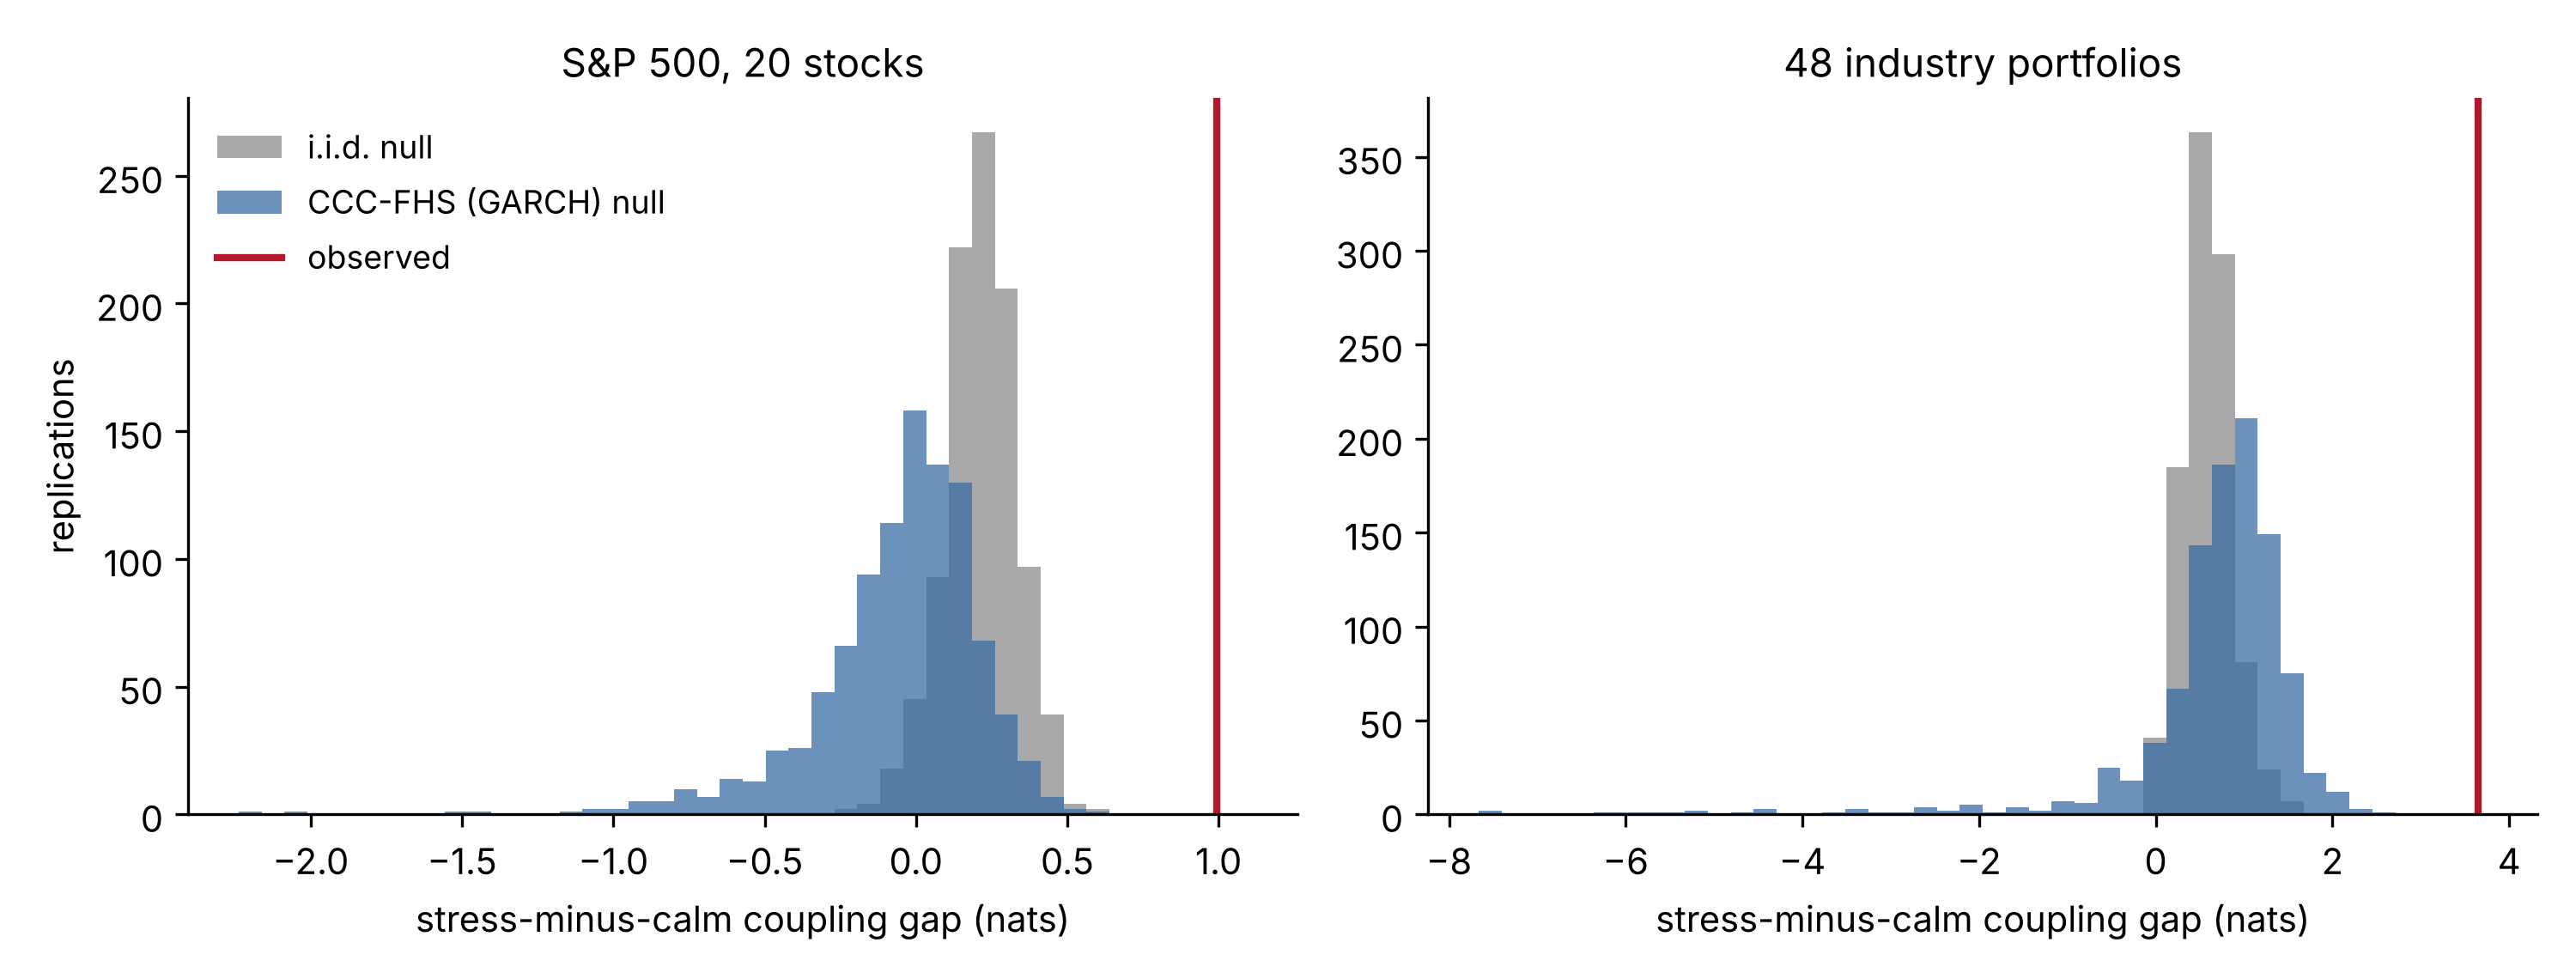
\includegraphics[width=\linewidth]{figures/fig_null_distributions.png}
\caption{Coupling under stress against two placebo nulls. Each panel shows
the stress-minus-calm gap in coupling $C$ (nats; positive means assets couple
under stress) for the observed data (vertical line) and for \nRep\ replications
of the i.i.d.\ null and of the CCC-FHS (constant-correlation GJR-GARCH) null.
Left: twenty S\&P~500 stocks, 1990--2022. Right: 48 industry portfolios,
1990--2026.\\
\emph{Alt text:} Two histograms. In each, the two null distributions sit well
to the left of a vertical line marking the observed coupling gap, the
GARCH null slightly to the right of the i.i.d.\ null.}
\label{fig:null}
\end{figure}

\begin{figure}[p]
\centering
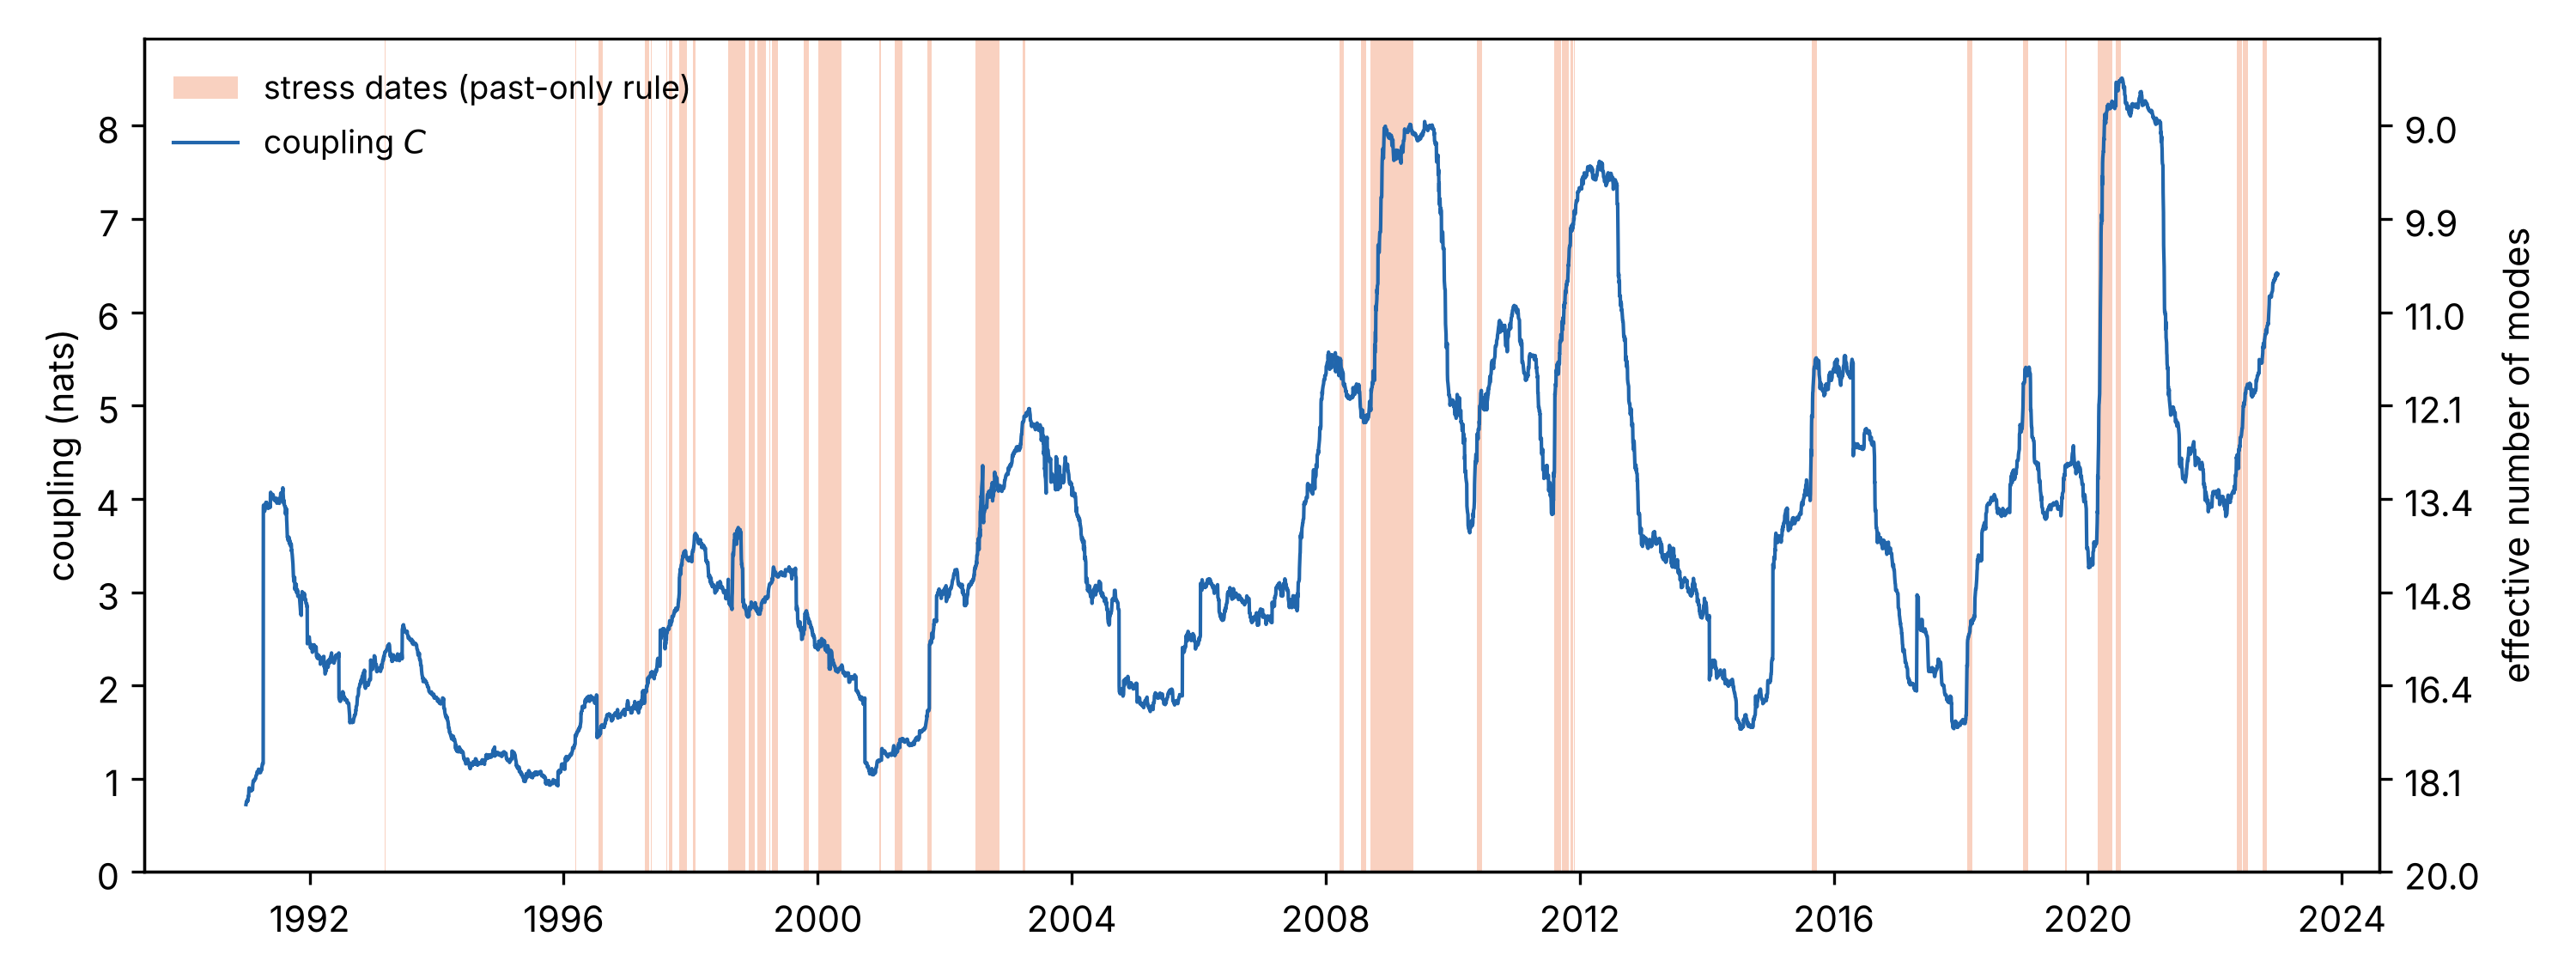
\includegraphics[width=\linewidth]{figures/fig_coupling_series.png}
\caption{Coupling of twenty S\&P~500 stocks, 1990--2022. Rolling 252-day
coupling $C=-\tfrac12\log\det R$ (nats, Ledoit--Wolf estimator), with
past-only stress dates shaded. The right axis gives the effective number of
risk modes $N\exp(-2C/N)$.\\
\emph{Alt text:} A time series of coupling with peaks in 2008 and 2020,
aligned with shaded stress periods.}
\label{fig:series}
\end{figure}

\end{document}
